\clearpage
\subsubsection{\olly + fields are packed by default}
\myindex{\olly}

Let's try our example (where the fields are aligned by default (4 bytes)) in \olly:

\begin{figure}[H]
\centering
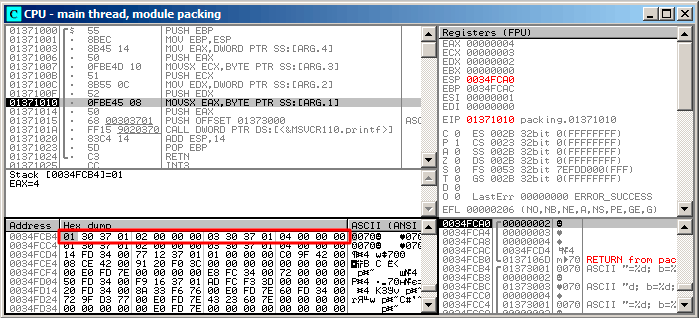
\includegraphics[scale=\FigScale]{patterns/15_structs/4_packing/olly_packing_4.png}
\caption{\olly: Before \printf execution}
\label{fig:packing_olly_4}
\end{figure}

We see our 4 fields in the data window.

But where do the random bytes (0x30, 0x37, 0x01) come from, that are next to the first (a) and third (c) fields?

By looking at our listing \myref{src:struct_packing_4}, we can see that the first and third fields
are \Tchar, therefore only one byte is written, 1 and 3 respectively (lines 6 and 8).

The remaining 3 bytes of the 32-bit words are not being modified in memory!
Hence, random garbage is left there.
\myindex{x86!\Instructions!MOVSX}

This garbage doesn't influence the \printf output in any way, because the values for it are prepared
using the \MOVSX instruction, which takes bytes, not words: 
\lstref{src:struct_packing_4} (lines 34 and 38).

By the way, the \MOVSX (sign-extending) instruction is used here, because 
\Tchar is signed by default in MSVC and GCC.
If the type \TT{unsigned char} or \TT{uint8\_t} was used here, 
\MOVZX instruction would have been used instead.

\clearpage
\subsubsection{\olly + fields aligning on 1 byte boundary}
\myindex{\olly}

Things are much clearer here: 4 fields occupy 10 bytes and the values are stored side-by-side

\begin{figure}[H]
\centering
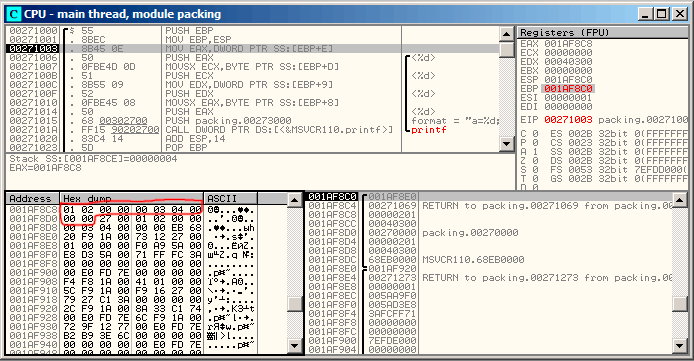
\includegraphics[scale=\FigScale]{patterns/15_structs/4_packing/olly_packing_1.png}
\caption{\olly: Before \printf execution}
\label{fig:packing_olly_1}
\end{figure}
